\documentclass[a4paper,10pt,onecolumn]{book}
% document preamble starts
\usepackage[colorlinks=true,linkcolor=black]{hyperref}
\usepackage{amsmath,array}
\usepackage{lipsum,blindtext,graphicx,verbatim}
%\hyperref


\title{Webinar on \LaTeX}
\author{Prateek Raj Gautam}
%\email{mailto:prateekrajgautam@gmail.com}


% document preamble ends


\newcommand{\code}[1]{$\backslash #1$}
\newcommand{\codee}[1]{$$ #1$$}


%main Document START here
\begin{document}
\frontmatter
\maketitle
%\newpage
%$L^AT_EX$
\tableofcontents
\mainmatter
\chapter{Day 1}

\section{Installation and basic tools}
Download TEXLIVE iso  from url \url{http://www.tug.org/texlive/}. Same iso image can be used on both linux and windows. Just mount it and run install command in the root directory and accept default options. It might take around 20 minutes to complete installation.
\subsection{Editors}
Although tex files can be edited in any basic text editor. just create a file with extension *.tex. you can create a new file newDoc.txt edit it save it and rename it as newDoc.tex so it can be used by tex or latex system.

However, to ease the process we will use TEXWORKS \url{https://github.com/TeXworks/texworks/releases} the default latex editor/compiler that comes with the texlive. This is the minimalist kind of software, in my opinion best for beginners. Later, you might want to try other editors like \url{https://www.texstudio.org/} or \url{https://www.texniccenter.org/}.

\subsubsection{Shortcuts for texworks}
\begin{table}[!htbp]
\begin{tabular}{p{.4\linewidth}|p{.4\linewidth}}
\hline
\ &\ \\
SHORTCUT&FUNCTION\\
\ &\ \\
\hline
$ctrl+t$&compile\\

$\left. ctrl+shift+\right]$& comment line\\
$\left. ctrl+shift+\right[$& uncomment line\\
\hline
\end{tabular}
\end{table}

\section{Skeleton file}
create tex file with
anyname.tex\\
type this code in it and save it.\\

\par
\noindent\rule{\linewidth}{1pt}
\begin{verbatim}
\documentclass{article}


\begin{document}

welcome

\end{document}
\end{verbatim}
\rule{\linewidth}{1pt}
after-compiling this file you will get a anyname.pdf file in the same folder like 


\framebox{
\begin{minipage}[t][5em][t]{.8\linewidth}
\maketitle
welcome
\vspace{5px}
\end{minipage}}
\vspace{5px}


$\backslash$documentclass should always be first line.\\
it can be used as any of the following each offer different set of options\\
$\backslash$documentclass\{article\}\\
$\backslash$documentclass\{book\}\\
$\backslash$documentclass\{letter\}\\
$\backslash$documentclass\{elsarticle\}\\



we can pass we extra options like selection of default paper size as \\
$\backslash$documentclass[a4paper]\{article\}\\
$\backslash$documentclass[letterpaper]\{article\}\\

we can select default font size as 10pt,11pt, or 12pt as\\
$\backslash$documentclass[a4paper,11pt]\{article\}\\

to print anything in document we write between $\backslash$begin\{document\} and $\backslash$end\{document\} .

the region before $\backslash$begin\{document\} is called document preamble and it is used to add different packages, function that alter the formatting to final document.


\section{Sectioning of document}
\subsection{section, subsection, and subsubsection}
\textbackslash$ section\{\}$\ $\backslash subsection\{\}$\ \textbackslash$subsubsection\{\}$
\subsection{paragraph, linebreak, and indentation}
\code{par}
\code{\backslash}
\code{noindent}
\subsection{chapter}
\code{chapter\{\}} to group \texttt{section} is
available in documentclass  \texttt{book} or \texttt{report}\\

\subsection{section, subsection subsubsection}
\blindtext
\section{Label and referencing}
$\ label{sec:lab}$\ $\ ref{sec:lab}$

\blindtext
%\subsection{hyperref}
%\subsubsection{colorlinks=true and linkcolor=black}
\section{Math}
\subsection{in-line and equation and eqnarray mode}
\codee{\$\mathbf{math}\$}
\codee{\$\$\mathbf{math}\$\$}
\codee{\backslash  [\mathbf{math} \backslash  ]}
\codee{\backslash begin\{equation\}  \mathbf{math} \backslash  end\{equation\}}


\subsubsection{eqnarray}
It uses \& to align equations and \\ to change line and add new eqn inside eqnarray environment
\codee{\backslash begin\{eqnarray\}  \mathbf{math} \backslash  end\{eqnarray\}}


\subsection{Symbols}
\codee{\backslash alpha \backslash beta  \backslash partial \backslash Delta \backslash gamma \backslash omega \backslash Omega \backslash vec\backslash nabla \backslash cdot \backslash vec B}
$$\alpha \beta  \partial \Delta \gamma \omega \Omega \vec\nabla \cdot \vec B $$


\subsection{Fractions sum integrals}
\code{frac\{num\}\{den\}}$\frac{num}{den}$
\code{sum  }$\sum$ 
\code{int}
$\int$

\subsection{Subscript and Superscript}
\begin{verbatim}
$a^2 $

$b_s$

$\sum_{i=0}^10$

$\int_0^\infty$

$a^2 $

$b_s$

$\sum_{i=0}^10$

$\int_0^\infty$
\end{verbatim}

\subsection{Dashes and minus}

\codee{a-b, a--b, a---b, \$-1\$}

a-b, a--b, a---b, $-1$


\subsection{Example equations}



$$\int^\infty_0{\frac{\overrightarrow{AB}}{\overrightarrow{C}\overrightarrow{D}}}$$




$$\vec{\Delta}.\vec{B}=0$$
$E=mc^2$
\[F=ma\]
$$\vec{F}=m\hat{a}$$
\begin{equation}
\vec{F}=m\hat{a}\end{equation}

\begin{eqnarray}
\vec{F}&=&m\hat{a}\\
\int\frac{d}{dt}y&=&\frac{\delta y}{\mathrm{d\qquad prateek} t} \qquad\qquad\qquad y\in \{ \mathbf{R}\}
\end{eqnarray}
\begin{equation*}
X(\omega) = 
\begin{cases}
1 &\text{se $\omega\in A$}\\
1250 &\text{se $\omega \in A^c$}
\end{cases}
\end{equation*}

$$
A=\left\{\begin{array}{rl}
A&=b\\c&=d\end{array}\right. \}
$$

$$ \vec\nabla \times \vec H = -\frac{\partial B}{\partial t}$$



\section{List, items and description}
\subsection{Un-numbered enumerate}
\subsection{Numbered itemize }
\subsection{Description}



\subsection{subsection}
\subsubsection{subsubsection}
In section \ref{sec:eqn} we describe eqn, in section \ref{sec:list} list



\section{list\label{sec:list}}

%\section{new addition}
%\section{Equations\label{sec:eqn}}

\begin{figure}[!ht]
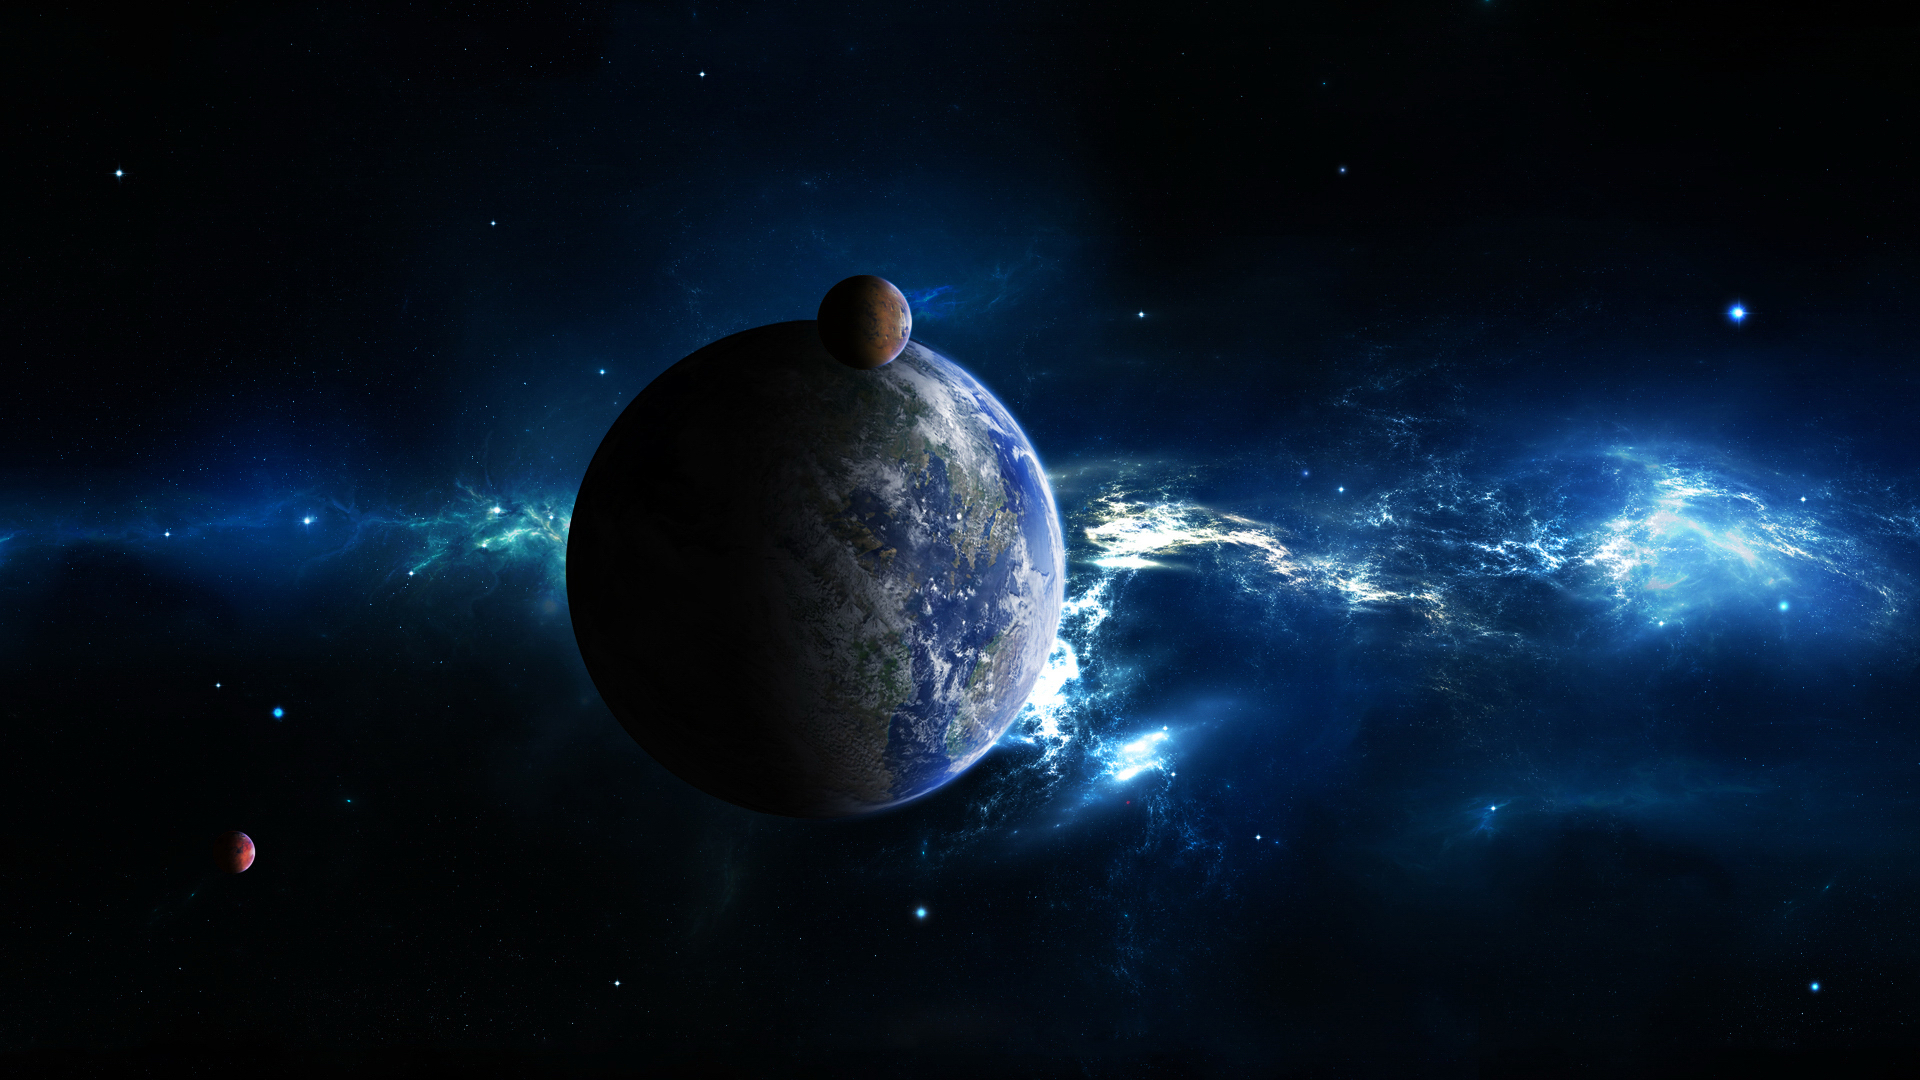
\includegraphics[width=\linewidth]{./images/1.jpg}
\caption{figure}
\end{figure}
\begin{figure*}[!ht]

\includegraphics[width=\linewidth]{./images/2.jpg}
\caption{figure* }
\end{figure*}






\section{table and tabular}
\begin{table}
\centering
\begin{tabular}{>{}p{3cm}|c|c|l}
\hline
hi sdg sd;f sdfllsdf adfdsf d df;glkd d sdfg;lk &dear&ssa&asd\\how &are you&&\\
\hline
hi&dear&ssa&asd\\how &are you&&\\
\hline
hi&dear&ssa&asd\\how &are you&&\\

\hline
\end{tabular}
\end{table}



\section{graphics picture and figure}

jo



\chapter{Day 2}

\section{Download and use IEEEtran \LaTeX template to convert article in to paper}

\end{document}
% main Document END here





%Comments start with %
% to compile press ctrl+t or hit the play button 